\documentclass[12pt,a4paper]{article}
\usepackage[utf8]{inputenc}
\usepackage[english]{babel}
\usepackage{xstring}
\usepackage{siunitx}
\usepackage{amsmath}
\usepackage{graphicx}
\usepackage[nottoc]{tocbibind} %Adds "References" to the table of contents
\usepackage{hyperref}
\usepackage[toc]{glossaries}
\usepackage{textcomp}
\usepackage{csvsimple}
\usepackage{pgfplotstable}
\pgfplotsset{compat=1.9}% supress warning
\usepackage{longtable}
\usepackage{xcolor,colortbl}
\usepackage{listings}
\usepackage[toc,page]{appendix}
\usepackage{fancyvrb}
\lstset{ %
language=C++,           % choose the language of the code
numbers=left,           % where to put the line-numbers
numberstyle=\tiny,      % the size of the fonts that are used for the line-numbers
basicstyle=\footnotesize    % the size of the fonts that are used for the line-numbers
}

\newcommand{\mc}[2]{\multicolumn{#1}{c}{#2}}
\definecolor{Gray}{gray}{0.85}
\definecolor{LightCyan}{rgb}{0.88,1,1}

\newcolumntype{A}{>{\columncolor{Gray}}c}
\newcolumntype{B}{>{\columncolor{white}}c}

% MODIFY NUMBERING OF TABLES AND PICTURES
\usepackage{chngcntr}
\counterwithin{table}{section}
\counterwithin{figure}{section}
\counterwithin{equation}{section}
\usepackage{floatrow}
\floatsetup[table]{capposition=top}

% HEADINGS AND MARGINS 
\usepackage{geometry}
 \geometry{
 a4paper,
 left=25mm,
 right=25mm,
 top=25mm,
 bottom=25mm,
 headheight=15mm,
 footskip=15mm,
 }
 

% PAGE STYLE SECTION
\usepackage{fancyhdr}
\pagestyle{fancy}
\renewcommand\sectionmark[1]{\markboth{\thesection\ #1}{}}
\fancyhf{}
\fancyhead[C]{\bfseries\leftmark}
\fancyfoot[C]{\bfseries\thepage}
\renewcommand{\headrulewidth}{0.5pt}% suppress the header rule

% INDENTATATIONS
\usepackage{indentfirst}
\setlength{\parindent}{0.75cm}

% FONT
\usepackage{times}

% UNIVERISTY LOGO TRIGGER
\usepackage{graphicx}

% TITLES OF PARTICULAR SECTIONS
\usepackage{titlesec}

\titleformat{\section}
    {\large\bfseries\itshape}
    {\thesection}
    {1em}
    {\MakeUppercase}
\titleformat{\subsection}
    {\large\bfseries\itshape}
    {\thesubsection}
    {1em}
    {}
\titleformat{\subsubsection}
    {\large\bfseries\itshape}
    {\thesubsubsection}
    {1em}
    {}
\titleformat{\paragraph}
    {\large\bfseries}
    {\theparagraph}
    {1em}
    {}
\titleformat{\subparagraph}
    {\large\bfseries}
    {\thesubparagraph}
    {1em}
    {}

\begin{document}

\begin{titlepage}
    \centering
    
\includegraphics[width=7cm]{logo.jpg} % also works with 
    \vskip1cm
    {\Large
        SILESIAN UNIVERSITY OF TECHNOLOGY\\
        FACULTY OF ELECTRICAL ENGINEERING\\
        \vskip0.5cm
        Department of Power Electronics, Electrical Drives and Robotics\\
    }
    \vskip1cm
    {\bfseries\huge
    Master's thesis\\
    }
    \vskip1cm
    {\bfseries\large
    To be determined \\
    }
    \vskip2cm
    {\large
    \begin{tabular}{p{4cm} p{10cm}}
    Student: & {\bfseries\Large Igor Aleksander JANKIEWICZ}\\
    Transcript no.: & 285947\\
        &   \\
    Type of studies: & Extramural studies (MSc programme)\\
    Field of study: & Electrical Engineering\\
    Programme: & To be determined\\
        &   \\
    Supervisor: & PhD. EEng. Andrzej Latko\\
    \end{tabular}
    }
    \vskip2.5cm
    {\large
    Gliwice 2020}
\end{titlepage}
\newpage\null\thispagestyle{empty}\newpage
\tableofcontents
\newpage\null\thispagestyle{empty}\newpage

\section{What is Energy Harvesting?}
Energy Harvesting is a process of using ambient energy by converting it into a usable form, i.e. electricity or heat. It is important to point out that energy harvesting has been around for quite a long time, since solar panels, wind turbines and water turbines are in constant use for a few decades, providing people with environmentally clean energy \cite{EnHv1}.
\vskip 5mm
There are some important issues related to any energy source that could be potentially used for harvesting. First of all, it is crucial to evaluate intensity and availability of that source. Subsequently, one should find out a cost-effectiveness of the solution as well as the influence of the harvesting process on the primary energy source \cite{EnHv1}.\par
\vskip 5mm
Vibration-based Energy Harvesting incorporates a number of different fields of study, i.e. material science, mechanics or electrical engineering, just to name a few. Last sentence implies that the analysis of a piezoelectric generator itself is not a straightforward process. The electromechanical response of this device relies thoroughly on the source of ambient energy \cite{EnHv2}.\par
\begin{figure}[h!]
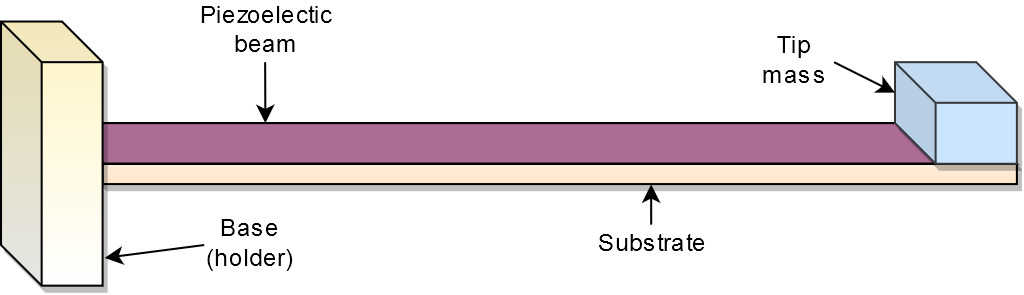
\includegraphics[scale=0.3]{beam1.jpg}
\end{figure}
\begin{table}[ht]
\small
\begin{center} 
\begin{tabular}{|c|c|c|c|c|}
\hline 
\textbf{Type} & \textbf{Conditions} & \textbf{Power Density} & \textbf{Area or Volume} & \textbf{Energy/Day} \\ 
\hline 
\hline
Vibration & $1m/s^2$ & $100\mu W/cm^3$ & $1cm^2$ & $8.64J$ (continuous vibration) \\ 
\hline 
Solar & Outdoors & $7500\mu W/cm^2$ & $1cm^2$ & $324J$ (sunny half a day) \\ 
\hline 
Solar & Indoors & $100\mu W/cm^2$ & $1cm^2$ & $4.32J$ (sunny half a day) \\ 
\hline 
Thermal & $\Delta T = 5 ^{\circ} C$ & $60\mu W/cm^2$ & $1cm^2$ & $2.59J$ (heat available for half a day) \\ 
\hline 
\end{tabular} 
\end{center}
\caption{Common data for some of Energy Harvesting Sources \cite{EnHv1}}
\label{tab:typdat}
\end{table}

\section{Operational amplifier selection}

Random citation \cite{EnHv1} embeddeed in text.

\newpage

\bibliography{bibliography} 
\bibliographystyle{ieeetr}

\end{document}
